%%%%%%%% IMPORTS %%%%%%%%%%%
\documentclass[a4paper, 12pt]{article}
\usepackage[francais]{babel}
\usepackage{graphicx}
\usepackage[utf8]{inputenc}
\usepackage[T1]{fontenc}
\usepackage{fancyhdr}
\usepackage[margin=1in]{geometry}
\usepackage{amsmath}
\usepackage{amssymb}
\pagestyle{fancy}
\newcommand{\Touche}[1]{\Ovalbox{#1}}
\usepackage{fancybox}
\usepackage{hyperref}
\hypersetup{
    unicode=false,          % non-Latin characters in Acrobat’s bookmarks
    pdftoolbar=true,        % show Acrobat’s toolbar?
    pdfmenubar=true,        % show Acrobat’s menu?
    pdffitwindow=false,     % window fit to page when opened
    pdfstartview={FitH},    % fits the width of the page to the window
    pdftitle={My title},    % title
    pdfauthor={Author},     % author
    pdfsubject={Subject},   % subject of the document
    pdfcreator={Creator},   % creator of the document
    pdfproducer={Producer}, % producer of the document
    pdfkeywords={keyword1, key2, key3}, % list of keywords
    pdfnewwindow=true,      % links in new PDF window
    colorlinks=true,       % false: boxed links; true: colored links
    linkcolor=black,        % color of internal links (change box color with linkbordercolor)
    citecolor=green,        % color of links to bibliography
    filecolor=magenta,      % color of file links
    urlcolor=blue           % color of external links
}
\usepackage{lscape}

%%%%%%%% PAGE PRINCIPALE %%%%%%%%%%%
\author{Benjamin \bsc{Moreau}, Jasone \bsc{Lenormand}}
\title{EZzik : logiciel d'apprentissage de la musique}

\begin{document}
\maketitle
\clearpage
\tableofcontents
\clearpage

%%%%%%%%%%% Benjamin
\section{Introduction} 
    Dans le cadre de notre cours  \emph{Interfaces homme-machine}, il nous est demandé de développer une petite application pour ordinateur permettant d'apprendre à lire une partition musicale. L'objectif principal du projet est de concevoir une interface de qualité pour ce logiciel puis de l'évaluer et de la critiquer. Ce logiciel devra être conçu à l'aide du langage de programmation \emph{C++} et de la librairie \emph{Qt}.
    
    Dans ce dossier, nous citerons les fonctionnalités de notre logiciel nommé \emph{EZzik}. Ensuite, nous intégrerons la \emph{storyboard} de l'application puis une présentation de \emph{l'interface Homme-Machine} et des différents choix que nous avons effectués sera faite. Enfin, Nous tenterons d'évaluer et de remettre en question notre interface en analysant les résultats de testes et avis extérieurs.

    Le paper-prototype est présenté à la section \ref{subsec:Paper-prototype}. le lien suivant : \href{https://youtu.be/iWcTD7AGAPs}{\emph{YouTube}} permet de le visionner.

%%%%%%%%%%% Benjamin
\section{Storyboard}
    \paragraph{}
    Avant de structurer l'interface ou encore de définir les fonctionnalités de l'application, il est important de savoir quel est le but du logiciel. En plus de montrer ce que recherche le client, le \emph{storyboard} est un bon moyen pour cerner le type d'utilisateur, l'environnement dans lequel l'application va être utilisé et surtout les besoins de l'utilisateur qui devront être comblés.
    \paragraph{}
    Dans un premier temps, nous avons donc constitué le \emph{storyboard} suivant :
     
    \begin{landscape}
    \begin{center}
    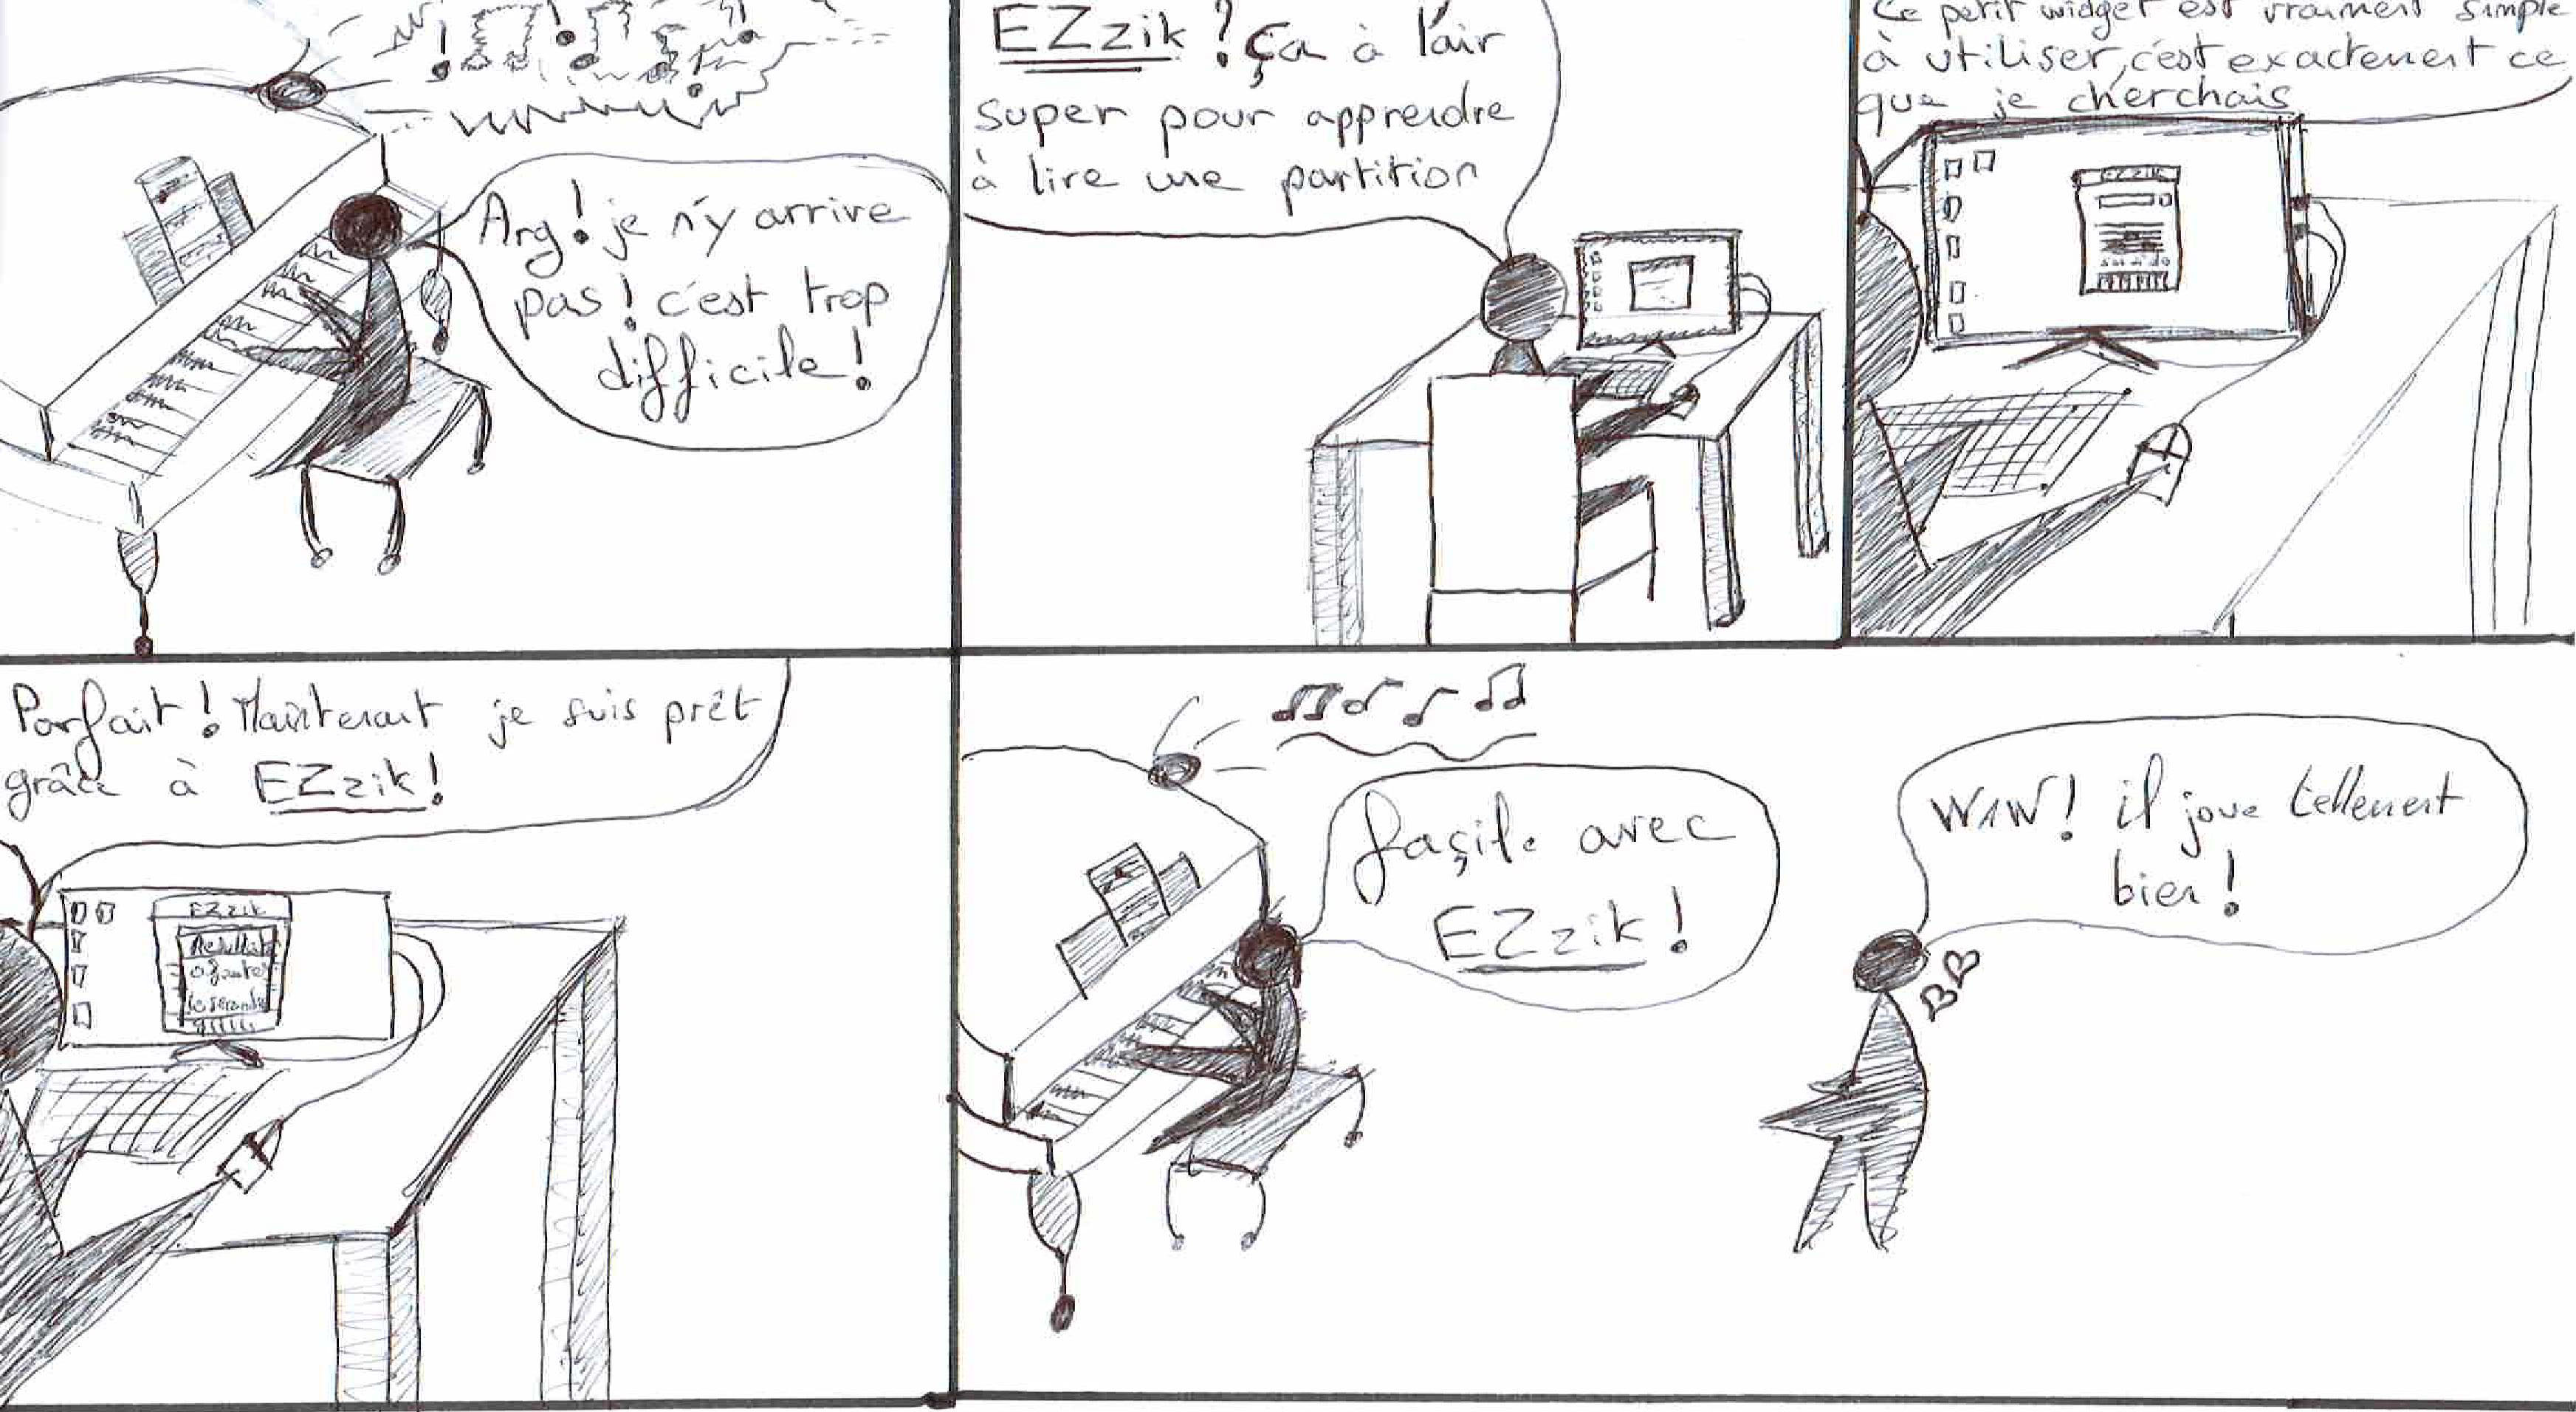
\includegraphics[scale=0.8]{storyboard_EZzik.jpg}
    \end{center}
    \end{landscape}

%%%%%%%%%%% Jasone
\section{Les Fonctionnalités de EZzik}
    \paragraph{}
    Afin de rendre l'apprentissage du solfège à la portée de tous, nous avons doté EZzik des fonctionnalités suivantes : Le programme affiche les notes d'une partitions à l'utilisateur. Celui-ci doit deviner l'emplacement de ces notes sur un clavier de piano (parmi deux octaves). Pour ce faire, il doit clicker sur la touche d'un clavier virtuelle, correspondante à la note courante. Un click sur une touche joue la note en question avec un son de piano.
    \paragraph{}
    Le chargement de différentes partitions à partir de fichiers texte est possible. En les mettant en dur dans la code, une fois l'utilisateur arrivé au bout de celles déjà proposées, il n'aurait pas été envisageable d'en rajouter ou même de les créer lui même. L'utilisateur peut également, à tout moment, changer de partition ou recommencer la courante et ce en un simple click sur un bouton.
    \paragraph{}
    Une correction indique à l'utilisateur les notes erronées et lui demande alors de recommencer celle pour les-quelles il s'est trompé. Quand toutes les notes ont été deviné, l'utilisateur est informé de ses performances tel que le temps passé à deviner les notes et son nombre d'erreurs.
    \paragraph{}
    Une aide sur l'interface et le fonctionnement du logiciel est à disposition de l'utilisateur en cours d'exécution de l'application.
    \paragraph{}
    Finalement, la fenêtre de l'application est entièrement modulable pour le confort de la vue de la personne utilisant l'application.

\section{Présentation de l'interface Homme-Machine}
    %%%%%%%%%%% Jasone
    \subsection{Choix d'interface}
    \paragraph{}
    L'interface peut être décomposée en trois parties principales. La première contient tous les boutons liés aux réglages de l'application. La seconde est dédiée à l'affichage des interactions entre l'utilisateur et l'application (incluant la partition et les notes entrées par celui-ci). La dernière comporte le clavier qui permettra à l'utilisateur d'interagir avec la seconde partie.
    
    \paragraph{}
    La première partie comporte un bouton \emph{Reset} permettant de recommencer directement la partition courante. Un \emph{ComboBox} permettant de choisir la partition. Un bouton \emph{Folder} ouvrant une interface de sélection du dossier contenant les partitions et un dernier bouton \emph{Info} affichant de l'aide sur la logiciel. Tout ces boutons ne concerne pas directement l'apprentissage du solfège qui est le but principal de l'application. C'est pour cela qu'ils ont été regroupé ensemble et qu'il occupe le moins d'espace possible dans l'interface. L'utilisateur est susceptible d'interagir avec eux à n'importe quel moment, c'est pour cet raison que nous les avons gardé dans la fenêtre principale.
    
    \paragraph{}
    Le bouton \emph{Reset} comporte deux flèches vertes en cercle pointant l'une sur l'autre (icon très souvent utilisée pour cette tâche dans la majorité des applications). Le bouton d'ouverture de dossier est lui aussi vert et représente bien évidemment un dossier. La couleur du dossier de ce genre de boutons varie très souvent d'une interface à une autre. Par exemple sous \emph{Windows} il est jaune, sous \emph{Ubuntu Mate} orange et sous \emph{Mint} il est vert. Étant sous \emph{Mint} où la couleur dominante est le vert, nous avons choisis vert également. De plus, cet couleur est en harmonie avec le bouton \emph{Reset} et permet de garder un lien entre les boutons de paramétrage. Le bouton \emph{Info} quand à lui est bleu et contient un point d'interrogation afin de respecter les conventions quand à son apparence dans la majorités des applications.
    
    \paragraph{}
    La second partie contient les notes à deviner de la partitions et les notes entrées par l'utilisateur au format textuel. Étant la plus importante en terme d'interactions, c'est elle qui prend le plus de place et qui se trouve au centre de l'interface. Les notes fraîchement entrées et non corrigées sont noir pour représenter la neutralité et pour qu'elles apparaissent comme dans une vraie partition. Les altérations de notes se situe en bas à gauche de celle-ci, une fois de plus pour respecter les conventions d'une véritable partition. Quant une note corrigée est fausse, celle-ci est remplie d'une couleur rouge et dans le cas inverse d'une couleur verte. Le rouge étant associé à une erreur lors des corrections, il est alors facile de conclure que les notes vertes sont correctes.
    
    \paragraph{}
    Les notes textuelles ont exactement les mêmes codes couleurs que les vrais notes afin de garder un lien logique entre celles-ci. Quand un de ces champs texte prend un couleur, on préserve un liserait noir autour pour une bonne visibilité sur le fond blanc et pour que le texte ressemble à sa note (note ayant aussi une couleur entouré d'un cercle noir).
    
    \paragraph{}
    Une barre traverse la note que l'utilisateur doit deviner à un instant t pour qu'il puisse sans efforts savoir où il est rendu dans l'exercice. 
    
    \paragraph{}
    La troisième partie représente un clavier de piano sur deux octaves. Une fois de plus, la couleur des touches et leur taille correspondent à celles dans la réalité pour facilité le passage de l'application à une mise en pratique réelle. Quand une touche est clickée, celle-ci change légèrement de couleur vers un ton gris afin que l'utilisateur sache clairement quelle note il a enfoncé et n'est pas de doute quand à la prise en compte de son action par l'application. De plus, le son de la note qu'il aurait entendu sur un vrai piano est joué à se moment afin d'ajouter un apprentissage auditif au visuel.
    
    \paragraph{}
    Une nouvelle fenêtre, complètement indépendante de la première apparaît quand l'utilisateur presse le bouton d'aide. De cette manière, si il veut garder l'aide en même temps qu'il joue, il peut placer la nouvelle fenêtre à côté de la principale et facilement faire passer sont regard de l'une à l'autre.
    Quand à l'organisation de cette fenêtre d'aide, elle contient sur la gauche une image de l'application découpé en sous parties par une couleur rouge vive et un numéro de partie afin de créer une rupture avec les couleurs de l'application. Ainsi, l'utilisateur comprend tout de suite que ces cadres et numéros rouges ne font pas partie de l'application mais sont une information supplémentaire liée à l'aide.
    
    \paragraph{}
    Dans la partie gauche, on retrouvera en gros le numéro de chaque parties du découpage avec une explication de la partie en question et son fonctionnement.  Le découpage se fait verticalement ce qui donne à la fenêtre une forme étendue sur l'horizontale de l'écran, plus facile à lire selon nous.
     
    \paragraph{}
    L'application en elle même est redimensionnable en étirant la fenêtre à la guise de son utilisateur. Tout les composants vont alors se redimensionner et s'agrandir en continuant d'occuper au maximum la fenêtre pour ne pas laisser de vide. Ainsi, les personnes ayant du mal à voir correctement certaine partie pour utiliser l'application d'une manière plus confortable.
      
    \paragraph{}
    Nous avons utilisé une seule police d'écriture et le texte est suffisamment grosse pour être très facilement lisible. Il y a en tout trois couleurs. Le bleu associé à l'aide, celui ci n'ayant aucun rapport direct avec le reste de l'application. Le vert quand à lui concerne uniquement les actions positives et le rouge une erreur de l'utilisateur. Les partie non colorée représente quelque chose de statique où à caractère neutre quand à sa véracité.
    
    \paragraph{}
    De manière générale, l'interface est sobre et épurée afin d'éviter toute information parasite et de ne pas perdre l'utilisateur. Elle est également très réactive et les actions s'enchaîne sans latence ce qui est plutôt agréable au niveau de l'utilisation.
    
    %% pistes pour la rédaction de cette partie %%
    %% avec citation du cours                   %%
    %% fenêtre statistiques : changement de fenêtre est associé a l'accomplissement d'une tache %%
    %% coherence entre les deux fenetres
    %% organisation symetrique et balancée ! : notes prennent toute l'espace sur la partition donc centré !
    %% une seul police d'ecriture
    %% 2 couleurs pas plus : avec signification forte VERT et ROUGE
    %% bouton et menu déroulant look and fill de l'OS
    %% contraste élevé : ameliore la lisibilité
    %% pas de latences !
    
    %%%%%%%%%%% Benjamin
    \subsection{Paper-prototype}
    \label{subsec:Paper-prototype}
    
    \paragraph{}
    Avant de commencer le développement de notre application, nous avons créé un premier \emph{paper-prototype}. Les essais que nous avons effectués sur ce dernier nous ont permis de rectifier certains défauts et d'obtenir le produit fini disponible à la fin de cette section.
    \paragraph{}
    Dans un premier temps, les notes étaient corrigées au fur et à mesure de l'avancée de l'utilisateur. Cette fonctionnalité permettait à ce dernier d'adapter le choix de ses futures notes en fonction du résultat des précédentes. De plus, les couleurs vives utilisées pour la correction polluait l'affichage de la partition et pouvait donc déconcentrer l'utilisateur. Afin de limiter cet effet, nous avons décidé de corriger la partition lorsque la dernière note est jouée. Cette modification permet à notre application de se rapprocher visuellement de la lecture d'une vraie partition.
    
    Dans un second temps, notre interface n'affichait pas les notes jouées. Dans le cas ou ce dernier est débutant au piano, il ne pouvait pas savoir quelle note il venait de sélectionner. De plus, la correction ne lui permettait pas de savoir quelle note lui posait des difficultés. C'est dans cette optique que nous avons ajouté sous la partition un affichage répertoriant les notes jouées par l'utilisateur.
    
    \paragraph{}
    À la suite de ces corrections, un deuxième \href{https://youtu.be/iWcTD7AGAPs}{\emph{paper-prototype}} a été créé. Le scénario correspondant à un usage ordinaire du logiciel est disponible à l'adresse suivante : \href{https://youtu.be/iWcTD7AGAPs}{YouTube}

%%%%%%%%%%% Benjamin
\section{Évaluation de l'interface}
    \subsection{Procédure de test}
    \paragraph{}
    Pour évaluer notre interface, deux sujets ont accepté de tester l'application individuellement en notre présence. Avant de commencer, ils ont été informés de l'objectif de l'application sans être renseignés sur son fonctionnement. Le but de cette expérience est de savoir avec quelle facilité l'utilisateur se familiarisera avec l'interface du logiciel.
    \paragraph{}
    Avant d'effectuer une action, l'utilisateur doit énoncer a voix haute le résultat qu'il pensera déclencher. Au lancement de l'application un chronomètre est lancé pour évaluer le temps d'adaptation approximatif du sujet à l'application. Pendant que l'utilisateur essaye le logiciel, les mouvements et clics de souris sont observés et des notes sont prises. Ces observations vont permettre de repérer les \emph{points chauds} de l'interface où l'utilisateur a tendance à mettre la souris et cliquer.
    \paragraph{}
    Ce test a été effectué sur deux profils différents. Le premier utilise régulièrement un ordinateur tandis ce que le deuxième est un novice et est habitué à utiliser une tablette.
    \subsection{Résultat de l'expérience}
        \subsubsection{Premier sujet}
        \paragraph{}
        Au lancement de l'application, aucune partition n'est chargée. Cependant, l'utilisateur essaye de cliquer sur les touches du piano. Ensuite, la souris se déplace vers la liste déroulante mais aucune partition n'y es présente. Le sujet va donc naturellement cliquer sur le bouton pour importer les partitions. Ses mouvements ont été représentés par la figure suivante. Les points représentes les clics de souris.
        \begin{center}
        \includegraphics[scale=0.5]{ouverture.png}
        \end{center}
        \paragraph{}
        Sur la fenêtre suivante ci-dessous, l'utilisateur a tendance à vouloir sélectionner directement une partition. Cependant, le sujet habitué aux ordinateurs comprend tout de suite le fonctionnement et sélectionne rapidement le dossier.
        \begin{center}
        \includegraphics[scale=0.3]{import.png}
        \end{center}
        \paragraph{}
        Enfin, le choix de la partition dans la liste déroulante s'effectue sans problème et l'utilisation du piano et la lecture de la partition est naturelle. Un problème survient quand l'utilisateur trouve une note parmi d'autres comme sur la figure ci-dessous. Le sujet est gêné par la tête de lecture qui ignore la note déjà trouvée. Au bout de 2 essais, l'utilisation du logiciel est fluide. La fonctionnalité de remise à zéro est assimilée instantanément.
        \begin{center}
        \includegraphics[scale=0.5]{jeu.png}
        \end{center}
        Le premier sujet a rapidement maîtrisé l'application au bout d'environ 4 minutes.
        \subsubsection{Second sujet}
        \paragraph{}
        Au lancement de l'application, le deuxième sujet effectue des clics de souris semblables au premier sujet puis clic sur le bouton d'import de partition.
        \paragraph{}
        Sur la deuxième fenêtre, l'utilisateur ne comprend pas pourquoi il est impossible de choisir les partitions. Au bout d'un certain temps, le dossier est choisi et les partitions chargées. L'utilisation de la liste déroulante est plutôt naturelle et la fonction de remise à zéro est bien utilisée.
        \paragraph{}
        Enfin, l'utilisation du piano est compris mais la correspondance entre les notes écrites et représentées sur la partition n'est pas assimilée.
        \paragraph{}
        Le deuxième sujet a plus difficilement maîtrisé l'application au bout d'environ 10 minutes.

%%%%%%%%%%% Benjamin
\section{Conclusion}
    \paragraph{}
    Suite à l'expérience, on observe que plusieurs points de \emph{l'interface Homme-Machine} de notre application peuvent être améliorés.
    
    Afin de guider l'utilisateur au lancement de l'application, il serait préférable de griser le piano, la liste déroulante et le bouton de remise à zéro. Une autre solution consiste tout simplement à charger une partition par défaut afin que le logiciel soit  directement opérationnel.
    
    Ensuite, il arrive que l'utilisateur ne sache plus où il en est quand il échoue pendant plusieurs tours. Une solution serait d'indiquer le nombre d'essais qu'il a déjà effectué.
    
    Le choix du dossier de partition ne semble pas adapté au sujet qui n'est pas habitué aux ordinateurs. Si le client visé n'est pas un utilisateur avancé, il est préférable de faire une application plus simple avec moins de possibilités ou le dossier de partition est imposé. La liste déroulante serait alors complète au lancement de l'application.
    
    Enfin, aucun sujet a tenté de redimensionner la fenêtre. Après échanges avec les sujets, il semblerait que la taille par défaut de l'application est adaptée, mais qu'aucune information n'est visible concernant la possibilité d'agrandir la fenêtre. Il serait préférable d'insérer un petit élément dans le coin inférieur droit pour indiquer à l'utilisateur qu'il est possible de la redimensionner.
    

\end{document}